\chapter{Discussion}

This thesis started with the aim of exploring the automatic assembly of timber frame structures with industrial robotic arms. However, as the investigation progressed, unforeseen discoveries and the development of the Distributed Robotic Tool (DiRT) concept, prompted a shift in the research focus. The new findings expanded the scope of the study, going beyond the initial research questions that guided its early stages. Consequently, the original questions were augmented to address the emerging knowledge gaps, reflecting the dynamic and evolving nature of the research.

In the preceding chapters, I have presented the validation experiments, observations, and lessons learned in each development iteration, following the chronological order of their discovery. In this Discussion chapter, I will analyse the results with a focus on understanding recurring patterns, providing generalisable theories, and discussing implications. I will start by responding to the original research questions posed at the outset of the dissertation before expanding into other topics that extend beyond them. This expansion reflects my commitment to exploring the most pressing issues within the domain of construction robotics. Finally, I discuss the potential for the versatile Distributed Robotic Tool (DiRT) concept to be adapted for use in other construction systems beyond timber frame structures,

It is important to note that much of the reasoning and conclusions in this chapter are based on the observations presented in earlier chapters. Links to those sections will be provided where appropriate to avoid repetition, but readers are advised to read the development chapters first for a comprehensive understanding.

Additionally, readers should be aware that the inductive approach used to explain observations in this chapter is subjective and interpretive in nature. The aim is not to prove or disprove a hypothesis but to find meaning through observations, to formulate new problems, to clarify concepts, and to form new hypotheses.

\section{Response to Research Questions}


	\bful{1.What technologies are required to assemble time frame structures?}

The DiRT system developed in this thesis demonstrated a viable method to overcome the challenges of assembling timber frame structures outlined in the introduction \textit{(see Chapter \uline{2 Challenges and Research Goals})}. In particular, the use of modular assembly tools to apply high forces to the joints proved to be a reliable solution for overcoming misalignment \textit{(see \uline{2.1.4 Joint Alignment}) }and high assembly resistance \textit{(see \uline{2.1.1 Sliding Friction}, \uline{2.1.2 Tight Fitting Joints} and \uline{5.6.6 Clamping Joints with Chamfered Edges})}. The flexibility to attach tools where needed allows the system to assemble many types of structures with different joint types, jointing angles, and timber sizes, with and without fasteners. In addition, the local correction effect at each joint was found to be exploitable for preventing global error accumulation.

    \bful{2. What are the robotic end effectors needed to assemble the joints?}

The DiRT concept introduced a significant change to the traditional definition of robotic end-effectors, transforming them into hybrids that incorporate elements traditionally found in mobile robots, such as embedded controllers, batteries and wireless communication. The modular nature of these tools enables various implementations based on specific joint requirements. In this thesis, two families of assembly tools were designed for a variety of lap joints \textit{(see \uline{4.2.1 Lap Joint Classification by Assembly Direction}, \uline{5.2.1 Parametric Variations of Lap Joints}, \uline{7.3.1 Parametric Polyline Lap Joints} and \uline{7.3.2 Parametric Non-Planar Lap Joints})}. One closes a joint by clamping it from the outside \textit{(see 5.3.4 Lap Clamp CL3 Hardware)}, while the other tightens a screw through the joint's centre \textit{(7.3.11 SL1 Screwdriver Electronics)}. The different placement options of the two tools also showcase the flexibility of attaching the DiRT tools either on the robot side or on the stationary side. Both modes of operation are useful depending on the type of joint being assembled.

    \bful{3. Can the DiRT tools be general-purpose, or are specific to the type of joint being assembled?}

DiRT is a general-purpose concept that can be extended for assembling different types of joints and other structures. In general, large-scale assemblies, especially ones that require multiple joint alignments and closure, can benefit from using DiRT. The only essential component of a DiRT tool is the docking adapter for the robotic arm to manipulate it. 

A DiRT tool does not even have to contain an active actuator. For example, the temporary scaffolding \textit{(see \uline{8.3.2 Scaffolding Support During Assembly})} used in the CantiBox can be converted to a DiRT tool \textit{(see \uline{10.3.1 Designing new DiRT tools}) }for it to be installed robotically.

\bful{4. Is the accuracy of a typical industrial robot sufficient to assemble timber beams with joints? Is it necessary to develop sense, alignment and compensation methods to overcome misalignment?}

There are a few types of alignment problems that are relevant to robotic timber frame construction. The first is pairwise alignment between two joints. This requires extreme accuracy because the joints are typically designed to be tight-fitting with no misalignment tolerance. During the development, this is shown to be solvable by the use of high assembly force and chamfered joint edges. Thanks to the low stiffness of timber and the programmable compliance of the robotic arm, the two pairs can be guided into alignment. \textit{(see \uline{7.3.16 Compliant Control for Robotic Arm})}

The second alignment problem occurs when there are more than one joint being assembled at the same time. The partially-assembled structure can deform in different directions, creating an overconstrained scenario and a conflict among alignment directions for each joint pair. However, what was thought to be a problem turns out to be a beneficial property. Observation shows that the local corrective behaviour at each joint can correct the deformation on the already-assembled structure. This allows the use of strategically designed timber parts to prevent global error accumulation. \textit{(see \uline{7.1.1 Deformation-Awareness and Error Correction by Triangulation})}

The third alignment problems arise from the use of robotic arms to manipulate DiRT tools. The implementation is challenging because tight tolerance is required to successfully place them on or retrieve them from the partially-built structure. The problem is worsened by the large deformation often seen on the partially-assembled structure. To address this issue, a contactless camera-marker alignment method was developed. The test result shows that it can direct the robotic arm to correct large deviations and achieve good alignment. \textit{(see 7.3.14 Camera-Marker Alignment Correction System)}

In general, it is not possible to answer whether an alignment will be successful. Different alignment scenarios have different amounts of deviation depending on the robot pose, the state of the partial assembly and many other factors that are unique in each moment. The correction mechanisms used, whether passive or active, have different correction ranges and success rates. The complexity of this problem is detailed in \uline{Chapter 9 New Hypothesis - Probabilistic Model of Spatial Alignment Success}, with a newly developed model to relate the probability of success with predictable deviations.

\bful{5. How suitable is an industrial robotic arm for performing spatial timber assembly? How can they be optimised for construction purposes?}

The RFL robotic platform demonstrated sufficient accuracy in assembling the three demonstrators using active and passive alignment correction methods. The kinematic combination of a robotic arm and an overhead gantry effectively manipulated the DiRT tools and timber components spatially to perform the assembly tasks. It provided good reachability to bring long timber elements through small openings of the structure and to attach and detach tools from tight spaces. However, if robots can be designed with longer and slimmer forearms, it could improve reachability and design flexibility. \textit{(see \uline{5.6.10 Robot Collision Problems}, \uline{5.6.11 Robot Cables Problems} and \uline{6.3.3 Robot Cable Guides})}

The overhead clearance provided by the gantry proved beneficial for finding collision-free trajectories during motion planning. This is because the robot carrying long beams can easily traverse the space above the partially-assembled structures. Nonetheless, care is needed to ensure ground-level operations are reachable and executable by the robot. \textit{(see 7.3.10 Beam to Ground Connection)}

On the downside, these demonstrators have pushed the robotic arm to its payload limit. Given that the demonstrators were small compared to actual buildings, future implementations should address the payload issue for larger structures. While it may not be feasible to increase reachability and payload while keeping a robotic arm slim, operation speed is less critical for construction robots and could potentially be sacrificed to accommodate improvements in other areas.

Lastly, current industrial robotic arms cannot detect and correct deviations caused by body deformation. Due to the non-repetitive nature of construction, robotic repeatability is no longer the only relevant specification. Construction robots need to reach a target pose accurately regardless of configurations, and payloads and to achieve this on the first try \textit{(see \uline{9.2.3 Accuracy of Robotic Platforms})}. Therefore, future construction robots should consider sensors that can measure body deformation and total flange deviation in real-time. This will allow absolute accuracy beyond repeatability. 

\bful{6. How many robots are needed to assemble a building?}

The combination of a single robotic arm and an overhead gantry has proven sufficient for constructing all the demonstration structures. Adding more arms may improve productivity, but the effect may not be easily quantifiable due to the harmful effect of overcrowding the planning scene. Multiple robots in collaboration may also enable tasks that are currently not possible, such as holding long beams at two points, creating sub-assemblies, or providing temporary structural support.

\bful{7. How can computational tools support a robotic assembly process?}

Computational tools are essential in supporting robotic assembly processes. In this thesis, their primary function is to assist users in designing the sequence of the assembly process, planning robotic tasks, and visualising, validating, and executing them. 

The modelling method is similar to traditional CAD and CAM software, but includes the concept of a step-by-step assembly process. This allows the user to model the changing location of objects and robots during the assembly. Interactive design and evaluation workflow was found to be useful for designing the robotic process modelling. \textit{(see \uline{5.2.7 Motion Planning})}

The creation of the robotic programme consists of two main steps. The first step is task planning - to create a list of task descriptions that need to be executed. The second step is motion planning - to create robotic trajectories for the robotic motion tasks. These two steps can also be performed together and are known as task and motion planning (TAMP). It is not only a computationally expensive process to search for collision-free robotic motions but also a difficult formulation problem for designers to convert the design of a structure into task descriptions for the computational algorithms to compute. In order to address this, my collaborator YiJiang Huang and I created two different types of formulation methods that bridge the gap between designers and programmers. \textit{(see \uline{6.3.5.1 Task Planning with Flowchart} and \uline{8.3.5 Specifying Actions and Goals for TAMP with PDDLStream})}

Because TAMP is a stochastic search in a high-dimension space, it is common to set a search limit for the process to decide when to give up. If a solution can be found within the given time, the assembly is considered constructible, and its motions can also be visualised. \textit{(see \uline{5.2.7.4 MP as a design feasibility check})} However, in the context of timber frame construction, the assembly scene is often a congested space that makes it hard for the robot to manipulate long timber beams. It is not uncommon for TAMP to fail even after hours of search. \textit{(see \uline{5.5.3 Narrow Passage Problem}) }This creates frustration for designers to wait for long hours only knowing that something went wrong. A better approach is to use lower-fidelity checks that are faster to perform for a more efficient fabrication-aware design workflow. Even if the quality of the check is not perfect, it is good enough to provide early-stage feedback to the designers. \textit{(see \uline{question 9 below})}

\bful{8. Can robotic programmes be generated automatically based on assembly design?}

The non-repetitive nature of architectural construction makes process modelling and TAMP a tedious task. Even the assembly of a simple structure involves thousands of steps\textit{ (see \uline{6.3.5.2 Expanding Task Groups})}. The sheer number of unique assembly scenes, robot targets, and motion constraints make manual modelling infeasible. Therefore, it is highly desirable if the static model of a timber structure can be automatically converted to robotic programmes.

During the development, it was found that all of the robotic movement targets can be extracted from the design model using rule-based algorithms \textit{(see \uline{6.3.5.4 Compute Robot Targets})}, but some decision related to the robotic process have to be decided by a production engineer \textit{(see \uline{6.3.5.6 Process Visualization and Adjustment})}. For example, the number of simultaneously assembled joints for a specific beam can be inferred from its joint-neighbour relationship from the design model. The position of that beam before closure can then be inferred from the assembly direction of each of the mating joints. If those joints are clamped, the task list for attaching the clamps can also be inferred from the number of joints, their positions and their required clamp model. \textit{(see \uline{6.3.5.1 Task Planning with Flowchart}) }Unfortunately, these algorithms are problem specific and are likely to require manual redesign when the assembly logic is changed. 

In some cases, the inference rule may contain more than one possibility for a decision, for example, the position where the robot holds a beam. In this thesis, the production engineer made the decision \textit{(see \uline{6.3.5.3 Process Parameters})}. However, it is possible that some rule-based or search-based algorithms can be developed in the future to make these decisions automatically. For example, during the design of the HyparHut and CantiBox, simple rule-based algorithms were tested and have been shown to reduce manual input to minimal. The remaining decisions are likely to be fully automatable if better modelling and automatic checks are developed, such as automatic deviation analysis\textit{ (see \uline{9.2 Estimating Deviations})}.

In addition, I have found that the data structure of the static model has a large influence on the difficulty when creating these inference algorithms. For example, how neighbour relations are described, and how beam and joint information is stored \textit{(see \uline{5.3.13 Assembly Model Data Structure and Functions})}. While a working data structure is developed for the timber assembly problem in this thesis, more work is needed to understand if it can be generalised. 

\bful{9. How will design validation be performed?}

Existing timber construction practice is typically concerned with structural validation (at both global and joint level) and CNC fabrication validation (to make sure joint details can be machined). While these validations are still required, the added robotic assembly process requires specialised validation to make sure it can be planned and executed. 

Practical experience has shown that some validation checks can be performed during design time with very fast feedback. This include: 

\begin{itemize}
	\item Infeasible assembly direction because of geometrical interlock

	\item Robotic payload limit \textit{(see \uline{7.5.5 Heavy Beam Caused Robot Overload})}

	\item Robotic reachability (IK + CC) \textit{(see \uline{7.3.21 Fast Design Validation with IK Check})}

	\item Collision between parts at keyframes

	\item Availability of assembly tools for all mating joints

\end{itemize}
On the other hand, TAMP is a much slower process that cannot provide real-time feedback to the designer. For example, it takes approximately 10 hours to compute TAMP for each demonstrator. The workflow feels like a ‘compile’ process to the designer, similar to the compile process in software development. The designer can only know for certain if the design will be constructible after a long wait \textit{(see \uline{5.2.7.4 MP as a design feasibility check})}. Moreover, due to the highly coupled and linear planning scene, even small design changes necessitate the re-computation of TAMP.

In order to address this, my collaborator and I have discovered different types of validation checks that can be performed, depending on the affordable time. This multiple level-of-detail validation process appears to be a practical approach to evaluating a design. The checks in increasing level of accuracy are:

\begin{itemize}
	\item Collision Check (< 1 minute)

	\item IK + CC (a few minutes) \textit{(see \uline{7.3.21 Fast Design Validation with IK Check})}

	\item LMG Planning (10 to 15 minutes) \textit{(see \uline{7.3.22 Planning Order by Motion Group})}

	\item Motion Planning (a few hours) \textit{(see \uline{6.3.7 Non-Sequential Planning Order})}

\end{itemize}
	\bful{10. What are the design constraints resulting from an automatic assembly process?}

In this thesis, DiRT tools have been developed for lap joints only and therefore the demonstrators are also designed exclusively with lap joints. While there are certain design constraints found during demonstrator design, it is hard to evaluate whether these constraints are caused by the specific tool implementation, the absence of other joint types, or if they represent a fundamental limitation with the DiRT concept itself. Especially because DiRT is an open system and new tools can always be added to solve a specific problem.

The only notable non-generalisable limit of the DiRT concept is the requirement for the tools to be attached to the structure or on the part being assembled. This restricts their attachment points to positions with sufficient stiffness to support the tools \textit{(see \uline{5.6.4 Unstable structure during assembly})}. It is easy to speculate that timber sizes smaller than those used in the demonstrations may struggle to hold the tools in place. Since it is unlikely that the DiRT tools can be made significantly lighter, the assembly process could potentially be scaled up, but scaling down may be challenging.

\bful{11. Can joint details be adapted to make automatic assembly easier?}

There are a number of construction details that are used to facilitate automatic assembly. In general they can be grouped into two types based on the intended purposes. The first type of details are for alignment correction, such as the chamfered edges in the lap joint for correcting pairwise alignment, and the fiducial markers added on the timber surfaces for camera vision \textit{(see \uline{7.3.14 Camera-Marker Alignment Correction System})}. The second type of details is used for registration, such as the registration holes machined on the beam that helps alignment with the robotic gripper and for the DiRT tools to be attached correctly \textit{(see \uline{4.3.1.2 Gripper for Hanging Clamp} and \uline{7.3.8 Parallel Gripper PG1500 for Long Beams})}.

In general, when designing construction details to facilitate automatic assembly, it is essential to examine whether that detail can be fabricated easily. In the case of timber construction, its compatibility with an automatic joinery machine is essential. In addition, reductive features such as registration holes and chamfered edges may have negative impact on structural performance and should be carefully studied.

	\bful{12. How will an automated timber construction process be implemented? What are the new domain experts and their responsibilities?}

\end{enumerate}
Considering the significant capital investment required for a large-scale robotic platform, it is essential for a DiRT system to be reusable across multiple projects with minimal modifications. A practical implementation would likely involve the development of an initial system prototype, similar to the one demonstrated in this thesis, which would be progressively improved over time. As the initial system becomes operational, additional DiRT tools, scaffolding elements, and sensors can be incorporated from project to project, thereby expanding the range of joint types and building components that can be assembled.

Based on the experience gained from operating the system, it is possible to speculate on the various domain experts needed during this expansion phase. Generally, some roles would be more focused on generic system design, while others would be responsible for executing projects and making project-specific modifications.

\begin{itemize}
	\item \textbf{System designer (CAD / CAM)}

\begin{itemize}
	\item Create modelling tools for designers in CAD environment 

\begin{itemize}
	\item Create parametric models of beams and joints \textit{(see \uline{7.3.1 Parametric Polyline Lap Joints})}

	\item Create design validation algorithms \textit{(see \uline{6.3.4 Design Software Implementation in Rhino Python})}

\end{itemize}
	\item Formulate assembly logic as TAMP problems

\begin{itemize}
	\item Create task planning flowcharts \textit{(see \uline{6.3.5.1 Task Planning with Flowchart})}

	\item Create an action-state description for automatic TAMP \textit{(see \uline{8.3.5 Specifying Actions and Goals for TAMP with PDDLStream})}

\end{itemize}
	\item Create process visualisation and reporting tools for designers, engineers and operators. \textit{(see \uline{6.3.5.6 Process Visualization and Adjustment})}

\end{itemize}
	\item \textbf{System designer (Robotic)}

\begin{itemize}
	\item Create high-level controllers for integrating and synchronising different controllers of robotic platforms, DiRT tools and sensors. \textit{(see \uline{5.3.12 Clamp Controller (L2)} and)}

	\item Create software for on-site operators to execute pre-planned robotic tasks, monitor progress, and allow certain reactions to on-site conditions. \textit{(see \uline{6.3.8 Standalone Process Execution Controller})}

	\item Design active and passive alignment correction mechanisms. \textit{(see \uline{7.3.14 Camera-Marker Alignment Correction System})}

\end{itemize}
	\item \textbf{System designer (Hardware)}

\begin{itemize}
	\item Design and fabricate DiRT tools

	\item Create digital twin models for the DiRT tools for integration into modelling, planning and control software. 

	\item Adapt the on-site robotic platform (gantry and arms arrangement) for project-specific requirements and site conditions. 

	\item Coordinate with the site operation manager, site safety engineer, and system integrator.

\end{itemize}
	\item \textbf{Production engineer}

\begin{itemize}
	\item Make process decisions and perform assemblability validation

\begin{itemize}
	\item Design temporary foundation \textit{(see \uline{7.3.10 Beam to Ground Connection})}

	\item Design temporary scaffolding positions \textit{(see \uline{8.3.2 Scaffolding Support During Assembly})}

	\item Decide grasp pose and assembly sequence \textit{(see \uline{6.3.5.6 Process Visualization and Adjustment})}

\end{itemize}
	\item Provide design feedback and suggestions to designers for resolving production problems.

	\item Provide feedback to system designers if new hardware or software is needed for project-specific requirements.

\begin{itemize}
	\item New joint type \textit{(see \uline{7.3.2 Parametric Non-Planar Lap Joints})}

	\item New building element type

	\item New assembly tool or sensor

	\item New scaffolding method

\end{itemize}
	\item Create robotic programme \textit{(see \uline{6.3.5 Process Design Workflow} and \uline{8.3.5 Specifying Actions and Goals for TAMP with PDDLStream})}

	\item Create CNC fabrication data for timber components \textit{(see \uline{5.6.1 Execution Plan} and \uline{7.5.1 Execution Plan})}

	\item Create production schedule, resources list and cost estimation.

\end{itemize}
	\item \textbf{Operator}

\begin{itemize}
	\item Monitor the automatic system and handle unexpected problems \textit{(see \uline{7.5.7 Screwdriver Dislodge Incident} / \uline{7.5.6 Screwdriver Tip Misalignment})}

	\item Perform machine tending and designated manual tasks 

\begin{itemize}
	\item Sort incoming delivery and check for defects \textit{(see \uline{7.5.3 Missing Cut Problem})}

	\item Load timber parts to the system

	\item Perform manual assembly tasks \textit{(see \uline{8.3.2 Scaffolding Support During Assembly})}

\end{itemize}
	\item Perform hardware inspection and maintenance

	\item Provide feedback to the production engineer and system designer about potential process improvement

\end{itemize}
\end{itemize}

\section{Risk Assessment of Robotic Processes}

During the demonstrations, there were multiple incidents where the automatic process failed due to deviation and misalignment. While most of these incidents were minor issues detected by the operator and resolved through manual adjustments, two incidents involving close calls of dropping DiRT tools raised concerns about operational safety and potentially expensive damages. \textit{(see \uline{8.5.6 Clamp Fall Incident} and \uline{7.5.7 Screwdriver Dislodge Incident}) }

In any process, there is always a chance that a task may fail, sometimes even in unimaginable ways. During the design of the clamp gripper, the main concern was to ensure that the clamp was secured during the attach operation before the docking adapter unlocks. To address this, an operator pause was introduced in the automatic process for the operator to visually confirm proper clamp attachment. Additionally, the spring-loaded clamp gripper is designed to passively hang on the structure even without power. However, the \textit{Clamp Fall Incident} happened during a different operation that was not considered high risk - the placement of a beam into the clamp jaws. The transferring beam deviated from its planned path, collided with the clamp jaw, and pushed open the spring-loaded gripper. This incident revealed the limitations of the original risk assessment and imagination and highlighted that no process could be completely reliable.

The importance of sensing failure can also be seen in the \textit{Screwdriver Dislodge Incident}. The problem could have been prevented if there had been a way to sense misalignment or when the screw tip failed to enter the hole. In fact, the inclusion of a camera had been considered during development, but the implementation was deemed too complex, and the idea was abandoned. In retrospect, even a basic camera installed on the screwdrivers could have helped the operator notice the anomaly and stop the automatic process. 

Based on the experiences gained during this thesis, several best practices and design principles are concluded that may benefit the future development of DiRT:

\begin{itemize}
	\item Conduct risk assessments for every step of the robotic process to anticipate problems and introduce risk mitigation.

	\item Anticipate the downstream implications and risk if a problem is not detected immediately. 

	\item Depending on the risk of a failure mode, decide if extra safety redundancy is needed.

	\item Provide means for error detection during operation. Ideally, with more than one method to detect an error. Honor Murphy's law.

	\item During development, include as many sensors as possible to avoid being blind to potential problems.

\end{itemize}

\section{Generalised DiRT system}

The discovery of the DiRT system started from an analysis of the joints used in timber frame structures. Apart from the fact that there are many joint types and irregular jointing angles, the most important observation is that these joints can be located in many different locations along the length of a beam. Moreover, there can be any number of joints that need simultaneous assembly. Through inductive reasoning, I determined that the most important quality of the assembly system is the flexibility for positioning tools wherever a joint is located. This effectively separated the problem of ``... many joint types and irregular jointing angles" from the problem of ``... many different locations". As such, the DiRT concept consists of two main hardware systems, each responsible for one of the two problems:

\begin{itemize}
	\item A set of modular tools, each of which $\ldots$

\begin{itemize}
	\item Can be attached to the joint area.

	\item Can perform one simple task effectively.

	\item Can be operated wirelessly and synchronously.

\end{itemize}
	\item A robotic manipulator / platform that $\ldots$ 

\begin{itemize}
	\item Can reach over, around, and into a partially assembled structure.

	\item Can attach tools to areas wherever they are needed.

	\item Can retrieve tools whenever they are no longer needed.

	\item Can transport workpieces to the work area.

\end{itemize}
\end{itemize}
None of these ideas are novel on their own. For example, robotic arms are commonly used to manipulate tools and workpieces and are able to pick and place objects. Automatic tool change is also a common operation on industrial robots for expanding the function of a single arm. The only distinct innovation in the DiRT concept is the ability for tools to operate while detached. This is rare in an industrial setting but has more similarities with mobile robots. However, the field of mobile robots is primarily concerned with creating autonomous devices that are capable of locomotion. In contrast, modular DiRT tools exhibit a distinctly simple design, as their relocation is performed by a high DOF robotic manipulator. This approach reduces the cost of the modular tools and simplifies their design to focus on the specific task at hand. 

While the development of each of these tools is presented in the previous chapters, the following section aims to describe the general properties of the tools and the robotic platform with the goal to inspire future development. For example, to design new assembly tools for more timber joint types, or even for other material and structural systems.

\begin{figure}[H]
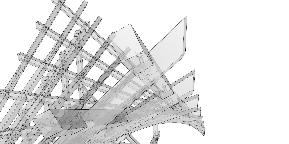
\includegraphics[width=15.92cm,height=8.96cm]{./images/image1.jpeg}
\end{figure}


The photo above shows the construction area before the beginning of the CantiBox. The DiRT Clamps and Screwdrivers are in the foreground. The robotic arm (right) can be seen approaching a parallel gripper. 

\subsection{Designing new DiRT tools}

DiRT tools are modular in nature which allows them to fulfil different types of roles. For example, the role of the robotic clamps is to create a high compressive force locally at the area of the lap joints; The role of the screwdriver is similar but the assembly force is pulled from the middle of the joint and is also able to place a permanent fastener. While assembly tools are the only type of tools being developed in this thesis, it is possible to develop other types of DiRT tools based on the experience gained from this thesis. 

This section presents a systemic design approach for designing new DiRT tools. In order to demonstrate the design procedures and considerations, I will attempt to redesign the temporary scaffolding in CantiBox (see photo below) such that it can be attached and detached automatically. I refer to this process of converting existing manual tools to a DiRT tool - DiRTify or DiRT-ification.

\begin{figure}[H]
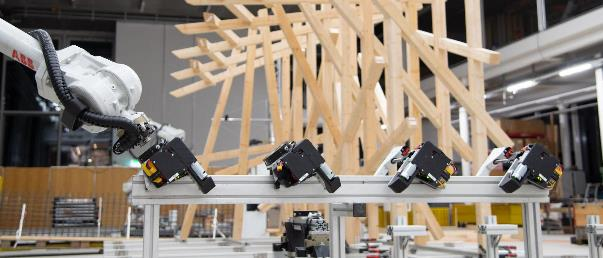
\includegraphics[width=15.92cm,height=8.96cm]{./images/image2.jpeg}
\end{figure}


The design process starts by drafting the specifications of the tool, which corresponds to two main operational aspects - the task to be completed and how the tool is attached. The table below contains an example of the specifications drafted for the DiRT scaffolding:

\begin{table}[H]
\begin{adjustbox}{max width=\textwidth}
\begin{tabular}{p{3.52cm}p{12.35cm}}
\hline
\multicolumn{1}{|p{3.52cm}}{{\footnotesize \textbf{Features to identify}}} & 
\multicolumn{1}{|p{12.35cm}|}{{\footnotesize \textbf{Example: Hypothetical DiRT-ified temporary scaffolding }}} \\ 
\hline
\multicolumn{1}{|p{3.52cm}}{{\footnotesize Task to be completed}} & 
\multicolumn{1}{|p{12.35cm}|}{\begin{itemize}
	\item {\footnotesize Provide support between two already-assembled timber elements. } \newline
\begin{itemize}
	\item {\footnotesize The two elements are always joined by a planar joint. } \newline
\begin{itemize}
	\item {\footnotesize No need to support non-planar joints } \newline
\end{itemize}
	\item {\footnotesize Since two elements are joined together, the addition of this scaffolding completes the third side of a rigid triangle.\par} \newline
\end{itemize}
	\item {\footnotesize If possible, one side of the scaffolding should be able to attach to the base platform.}\end{itemize}
} \\ 
\hline
\multicolumn{1}{|p{3.52cm}}{{\footnotesize Flexibility of the task}} & 
\multicolumn{1}{|p{12.35cm}|}{	\item {\footnotesize The two timber elements may be joined with different angles from 40 to 140 degrees.} \newline
	\item {\footnotesize The supporting bar length is fixed (different lengths should be available in the toolset but not adjustable on each tool)\par}} \\ 
\hline
\multicolumn{1}{|p{3.52cm}}{{\footnotesize Attachment Method}} & 
\multicolumn{1}{|p{12.35cm}|}{\begin{itemize}
	\item {\footnotesize Direction of attachment is to be determined, two possibilities exist:} \newline
\begin{itemize}
	\item {\footnotesize Enter from the gap between the two timber and pushed towards the timber joint.} \newline
	\item {\footnotesize Enter from the side of the two timber pieces, } \newline
\end{itemize}
	\item {\footnotesize Registration features may be needed on the timber at the attachment point. }} \\ 
\hline
\multicolumn{1}{|p{3.52cm}}{{\footnotesize How deviation affects the attachment process}} & 
\multicolumn{1}{|p{12.35cm}|}{	\item {\footnotesize Deviations between two beams are expected to be low because the scaffolding is attached while the weak beam is still held by the other robot. \par} \newline
	\item {\footnotesize Deviation analysis is performed to determine the following.} \newline
\begin{itemize}
	\item {\footnotesize Deviation of each attachment point from ground truth is <5mm @98$\%$ confidence. } \newline
	\item {\footnotesize Deviation between the distance of the two attachment point is <3mm @98$\%$ confidence. } \newline
\end{itemize}
	\item {\footnotesize The attachment process is not expected to push incorrect structures back to correctness. }\end{itemize}
} \\ 
\hline
\end{tabular}
\end{adjustbox}
\end{table}
{\footnotesize $\ast$ All numerical values in this table are for illustrative purposes only.}

When describing the task, it is necessary to analyse what kinematic actions are needed to perform the task, and if any essential parts are required. In this example, the scaffolding bar does not require any kinematic movement. However, in the screwdriver development, the screwdriver head and the pull screw were essential components.

When defining the geometrical flexibility of the task, be aware of its implications for the complexity of the tool. For example, if the scaffolding bar is to be extendable, an extra actuator is needed to do so. In general, it is best to avoid adding too much flexibility to the tool, as simplicity keeps the tool light and low cost. One potential opportunity for adjusting the dirt tool without adding an actuator is to use the robotic arm to adjust the tool. For example, we can design the scaffolding bar to be extendable, but the length adjustment is actuated by a push or rotation delivered by the robotic arm before the bar is being picked up.

When designing the attachment method, it is best to first identify the direction of which the tools are attached and detached. Ensure the robot can reach into the area to perform the attachment and the detachment scenario is not blocked by the presence of newly assembled parts. Based on the assembly direction, the attachment mechanism can be detailed. This mechanism needs to ensure good registration accuracy with the workpiece, good stiffness after attachment and should be protected against accidental release. The pneumatic parallel gripper and electric pin gripper are good examples that can be reused. Because the tool is to be attached to the partially-assembled structure by the robot, alignment-correction method is likely necessary to achieve a high success rate. Based on the experience of this thesis, the camera-marker method proves to be quite robust. 

Based on the specifications, a design study can generate different design options. The following list provides a guideline for important metrics to evaluate when deciding which option to pursue:

\begin{itemize}
	\item \textbf{Choice of power source} - Typically electric power is provided by an onboard battery. When the tool is attached to the robot, high-power electricity and pneumatic power can be provided through the docking adapter. Evaluate cost and power consumption per operation cycle.

	\item \textbf{Weight of the tool }- Perform additional deviation analysis for typical attachment scenarios to make sure the tools can be hung from their intended locations without causing excessive deformation.

	\item \textbf{Implementation complexity and cost - }Evaluate the choice of actuators and the required drivers and controllers. Typically, fewer actuators make the device simpler and lighter.

	\item \textbf{Chance of successful attachment - }Based on the alignment mechanism and the choice of alignment correction mechanism, estimate the allowable tolerance and correction range. Evaluate the chance of successful alignment for typical attachment operations using the alignment-correction model. 

	\item \textbf{Risk of collision} - Perform collision check for every key step during attachment, operation and detachment process. All collision objects should be considered, such as, robots, other tools, already-assembled structure, and ground foundation. If the tool is flexible to interact with geometrically different workpieces, perform multiple checks for each degree of freedom (at least one checks at each extreme of the flexibility and at the neutral position). Not all scenarios need to be collision free, for example, cases where multiple flexible dimensions are at their extremes can be exempted. The purpose of this evaluation is to get a sense of the design freedom. 

	\item \textbf{Command and control }- Evaluate whether the standard wireless command control framework can be used. Evaluate if bandwidth and latency is sufficient, especially if camera feed is required.

\end{itemize}
Finally it is necessary to consider the placement of the docking adapter. The position of the adapter directly determines the position of the robot flange and the position of the robot wrist when the tool is attached. For spherical wrist robots, such as the one used in this thesis, the wrist can be approximated by a sphere. A special property of these robots is that the sphere’s position relative to the flange does not change with the movement of Joint 5 or Joint 6. Therefore, we can use this sphere as a rule-of-thumb guidance to make sure there are no collisions with the parts being assembled.

In conclusion, the development of custom DiRT tools is a clearly defined mechatronics design process that is repeatable and adaptable to a wide array of applications. The systematic design approach presented here allows each new tool to be optimised for its specific task, while also maintaining compatibility with the overarching robotic system. By following these design guidelines and principles, engineers can create modular and versatile tools that extend the capabilities of the DiRT assembly system. 

\subsection{Robotic Platform}

The robotic platform used for DiRT operations is generic in nature. The specific implementation can be adapted to on-site conditions and the target building size. This is similar to how cranes of different size, payload capacity and base condition (stationary vs mobile) are selected in the current construction practice. 

The following table provides a list of robot specifications for DiRT operations that are crucial for achieving reasonable design freedom, efficiency, and safety during the construction process. It also includes how each specification can be determined according to the construction task in a generalised scenario. For timber frame construction, the values used for this thesis is included for reference, together with the recommended values concluded from the experience gained.

\begin{table}[H]
\begin{adjustbox}{max width=\textwidth}
\begin{tabular}{p{3.04cm}p{6.3cm}p{3.41cm}p{3.41cm}}
\hline
\multicolumn{1}{|p{3.04cm}}{\multirow{2}{*}{\parbox{3.04cm}{{\footnotesize \textbf{Specification}}}}} & 
\multicolumn{1}{|p{6.3cm}}{{\footnotesize \textbf{Generalised Construction Scenario}}} & 
\multicolumn{2}{|p{6.83cm}|}{{\footnotesize \textbf{Timber Frame Construction}}} \\ 
\hhline{~---}
\multicolumn{1}{|p{3.04cm}}{} & 
\multicolumn{1}{|p{6.3cm}}{{\footnotesize \textbf{Determination of Specification}}} & 
\multicolumn{1}{|p{3.41cm}}{{\footnotesize \textbf{Ideal Values}}} & 
\multicolumn{1}{|p{3.41cm}|}{{\footnotesize \textbf{Used This Thesis}}} \\ 
\hline
\multicolumn{1}{|p{3.04cm}}{{\footnotesize Robot Payload Capacity}} & 
\multicolumn{1}{|p{6.3cm}}{{\footnotesize Depends on weight of workpiece to be lifted}} & 
\multicolumn{1}{|p{3.41cm}}{{\footnotesize 100kg}} & 
\multicolumn{1}{|p{3.41cm}|}{{\footnotesize 60kg} \newline
} \\ 
\hline
\multicolumn{1}{|p{3.04cm}}{{\footnotesize Robot Wrist Torque}} & 
\multicolumn{1}{|p{6.3cm}}{{\footnotesize Depends on workpiece geometry and how it is held}} & 
\multicolumn{1}{|p{3.41cm}}{{\footnotesize 1000Nm}} & 
\multicolumn{1}{|p{3.41cm}|}{{\footnotesize 105Nm (Joint 6)} \newline
{\footnotesize 200Nm (Joint 4, 5)}} \\ 
\hline
\multicolumn{1}{|p{3.04cm}}{{\footnotesize Robotic DOF}} & 
\multicolumn{1}{|p{6.3cm}}{{\footnotesize At least 4 (top down construction) } \newline
{\footnotesize At least 6 (spatial construction)  \\ 9 (Ideal)}} & 
\multicolumn{2}{|p{6.83cm}|}{{\footnotesize 9 (3 Cartesian + 6 Robot Joints) Refer to \uline{5.2.2 RFL Robotic Platform}}} \\ 
\hline
\multicolumn{1}{|p{3.04cm}}{{\footnotesize Repeatability}} & 
\multicolumn{2}{|p{9.71cm}}{{\footnotesize Not very relevant. See Answer 5 of \uline{10.1 Response to Research Questions}}} & 
\multicolumn{1}{|p{3.41cm}|}{{\footnotesize 0.06 (Not very relevant)}} \\ 
\hline
\multicolumn{1}{|p{3.04cm}}{{\footnotesize Cartesian Accuracy}} & 
\multicolumn{1}{|p{6.3cm}}{{\footnotesize Depends on alignment requirements}} & 
\multicolumn{1}{|p{3.41cm}}{{\footnotesize 2mm (worst case)}} & 
\multicolumn{1}{|p{3.41cm}|}{{\footnotesize 10mm (worst case)} \newline
{\footnotesize 5mm (typical)}} \\ 
\hline
\multicolumn{1}{|p{3.04cm}}{{\footnotesize Robotic Arm Reach}} & 
\multicolumn{1}{|p{6.3cm}}{{\footnotesize Depends on the assembly task. } \newline
{\footnotesize E.g. Distance of one structural bay (structural assembly), height of one floor (facade assembly)}} & 
\multicolumn{1}{|p{3.41cm}}{{\footnotesize 2.5m}} & 
\multicolumn{1}{|p{3.41cm}|}{{\footnotesize 2.55m}} \\ 
\hline
\multicolumn{1}{|p{3.04cm}}{{\footnotesize Compactness}} & 
\multicolumn{2}{|p{9.71cm}}{{\footnotesize Depends on the assembly task, but in general: \\ Wrist - Small enough to attach and retrieve tools on structure\par} \newline
{\footnotesize Elbow - Small enough to reach into openings of partially-assembled structure}} & 
\multicolumn{1}{|p{3.41cm}|}{{\footnotesize Refer to the geometry of ABB IRB 4600-40/2.55.}} \\ 
\hline
\multicolumn{1}{|p{3.04cm}}{{\footnotesize Coordinate System}} & 
\multicolumn{3}{|p{13.12cm}|}{{\footnotesize Fixed coordinate reference for the entire job site (especially relevant for robot platforms with mobile base). Ideally aligned with the reference used by the surveyor.\par}} \\ 
\hline
\multicolumn{1}{|p{3.04cm}}{{\footnotesize Working Envelope of Gantry}} & 
\multicolumn{1}{|p{6.3cm}}{{\footnotesize Depends on size of the workpiece}} & 
\multicolumn{1}{|p{3.41cm}}{{\footnotesize 2m offset larger than building size}} & 
\multicolumn{1}{|p{3.41cm}|}{{\footnotesize 1.5m offset larger than building size}} \\ 
\hline
\multicolumn{1}{|p{3.04cm}}{{\footnotesize DiRT Docking Adapter}} & 
\multicolumn{2}{|p{9.71cm}}{{\footnotesize Standardised docking interface include power feedthrough (see next section - Docking Adapter for details)\par}} & 
\multicolumn{1}{|p{3.41cm}|}{{\footnotesize Schunk - SWA-040 (with pneumatic feedthrough)}} \\ 
\hline
\multicolumn{1}{|p{3.04cm}}{{\footnotesize Robot Impedance Control}} & 
\multicolumn{3}{|p{13.12cm}|}{{\footnotesize Impedance control is useful for allowing the robot to be slightly compliant during docking and passive correction.\par}} \\ 
\hline
\multicolumn{1}{|p{3.04cm}}{{\footnotesize Weather Protection}} & 
\multicolumn{2}{|p{9.71cm}}{{\footnotesize IP 67, rust protection on all weather exposed parts.}} & 
\multicolumn{1}{|p{3.41cm}|}{{\footnotesize Not required}} \\ 
\hline
\end{tabular}
\end{adjustbox}
\end{table}
\vspace{3\baselineskip}
The primary consideration in implementing the robotic platform is the kinematic arrangement. A popular approach, that is also used in this thesis, is the overhead gantry with an inverted robot arrangement. This arrangement offers overhead clearance to facilitate navigation in congested assembly areas. It is also the most common arrangement used in many of the integrated automated construction sites found in Japan \href{https://www.zotero.org/google-docs/?EF3GMo}{(Linner, 2013; Potter, 2022)} . Apart from its sturdiness, it provides other benefits such as attachment of vertical material transport robots and weather cover over the gantry.

There are alternative arrangements to the gantry-robot approach, one of which is crane-based robots, such as tower cranes or crawler cranes. They offer high lifting capabilities but face challenges controlling sway \href{https://www.zotero.org/google-docs/?Cg17jt}{(Neupert et al., 2010)} and rotation \href{https://www.zotero.org/google-docs/?xytkc0}{(Liang et al., 2017)}; Another alternative is robots based on articulating boom lifts, which provide good reachability but have lower payload capacities. These may be suitable for attaching and detaching DiRT tools but insufficient for lifting building components. 

In this thesis, the gantry-robot arrangement achieves a balance between accuracy, reachability and payload capacity suitable for timber frame assembly. However, for heavier construction components such as prefab-concrete and steel, it is likely that the role of heavy lifting and manipulating DiRT tools are distributed to two different robotic platforms, each optimised for their specific tasks.

In conclusion, the selection of an appropriate robotic platform for DiRT operations depends on the construction material and assembly process. While this thesis focused on the assembly of timber frame structures with integral timber joints, it is likely that actual on-site robotic platforms will need to accommodate a wider variety of components and processes. The specification of which will need to integrate and satisfy all requirements while maintaining flexibility.

\subsection{Docking Adapter}

In the previous sections, it was discussed that DiRT tools are modular and the robotic manipulator is generic. This leaves the interface between the two being the only unvarying aspect in a DiRT implementation. Much like the International Space Station's docking adapter, which unites and fosters cooperation among various space-faring nations, the DiRT docking adapter stands as a symbol of collaboration. It provides compatibility between new and old tools, those developed by different parties, and different robotic platforms deployed across diverse job sites.

The docking adapter is an automatic device that allows the robotic manipulator to pick up and attach a DiRT tool. A typical implementation consists of a pair of mechanical parts, one rigidly installed on the robot-side and the other one on the tool-side. An actuator within the mechanism performs locking or unlocking actions between the pair. The interface is often designed with tapered surfaces to correct for misalignments and to ensure docking repeatability. When docked and locked, the adapter serves as a strong and stiff mechanical connection between the arm and the DiRT tool and can provide electric and pneumatic power over the interface.

One of the most important specifications of the adapter is its payload capacity. Similar to the discussion in the previous chapter, the selection of a suitable capacity depends on how the entire DiRT system is integrated with other construction processes. Once this standard is set, all DiRT tool implementation is required to comply with its limitations. In this thesis, the docking adapter is implemented by adapting an existing off-the-shelf automatic tool changer \textit{(see \uline{5.3.5 Docking adapter})}. The specific model (SWA-040 by Schunk) was chosen because previous projects in the laboratory have donated them for reuse. Although it is slightly undersized for the timber beams, it was considered sufficient for demonstrating the DiRT system prototype. 

It is worth noting that the payload capacity of a docking adapter is directly related to its size. Therefore, overspecification of the adapter size does not only increase tool-side cost, but its physical size and weight can limit the performance of the tool. Therefore, in practice, it may be beneficial to have more than one adapter size. The largest of which is installed on the robotic platform and adapters between the adapters can be used to interface with smaller tools.

During the development of the automatic tool placement procedure, it was found that the docking tolerance of 2mm offered by the tool presented a challenge for robotic alignment. The solution was to add a camera on the robot side, target markers on the tool side, and develop an alignment algorithm to perform correction by moving the robot \textit{(see \uline{7.3.15 Camera-Marker Hardware on Docking Adapter})}. While this method proves to be highly successful, an alternative solution would be to redesign the mechanical interface to allow for more tolerance. In addition to the pneumatic feedthrough, it would also be beneficial to include a power feedthrough for charging the on-board tool batteries while the tools are being handled \textit{(see \uline{8.5.2.2 Combined Operation of DiRT Tools})}. 

\subsection{Wireless Communication System}

In order to communicate wirelessly with the DiRT tools, it is essential to have a high-performance and robust radio communication system. While there are many matured wireless communication systems like Wi-Fi and ZigBee, they do not fully address the unique challenges and requirements of DiRT systems in a construction environment. For example, ensuring signal reliability in a construction environment with many occlusions is challenging but essential to the robot process. As many of the DiRT movements require synchronising movements with multiple tools and robots, any dropped connection will result in an emergency stop, causing a disruption to the process. The following table lists the general requirements for a wireless communication system designed for DiRT operations:

\begin{table}[H]
\begin{adjustbox}{max width=\textwidth}
\begin{tabular}{p{2.33cm}p{8.25cm}p{5.34cm}}
\hline
\multicolumn{1}{|p{2.33cm}}{{\footnotesize \textbf{Property}}} & 
\multicolumn{1}{|p{8.25cm}}{{\footnotesize \textbf{Requirements}}} & 
\multicolumn{1}{|p{5.34cm}|}{{\footnotesize \textbf{Purpose}}} \\ 
\hline
\multicolumn{1}{|p{2.33cm}}{{\footnotesize Wireless Range}} & 
\multicolumn{1}{|p{8.25cm}}{{\footnotesize The system should offer an adequate communication range to cover the entire construction site. }} & 
\multicolumn{1}{|p{5.34cm}|}{{\footnotesize Avoid disruption to the automatic construction process.}} \\ 
\hline
\multicolumn{1}{|p{2.33cm}}{{\footnotesize Energy Efficiency}} & 
\multicolumn{1}{|p{8.25cm}}{{\footnotesize Energy-efficient endpoint on the tool-side as DiRT tools rely on battery power for extended periods of time.\par}} & 
\multicolumn{1}{|p{5.34cm}|}{{\footnotesize Extend DiRT battery operation time.}} \\ 
\hline
\multicolumn{1}{|p{2.33cm}}{{\footnotesize Low latency}} & 
\multicolumn{1}{|p{8.25cm}}{{\footnotesize Sufficiently low latency to ensure real-time control and monitoring of DiRT tools.}} & 
\multicolumn{1}{|p{5.34cm}|}{{\footnotesize Allow quick detection and responses to emergency conditions.}} \\ 
\hline
\multicolumn{1}{|p{2.33cm}}{{\footnotesize High Data Rate}} & 
\multicolumn{1}{|p{8.25cm}}{{\footnotesize Sufficiently high data rates to accommodate control commands and telemetry data from all active tools.\par}} & 
\multicolumn{1}{|p{5.34cm}|}{{\footnotesize Enable high telemetry frame rate.}} \\ 
\hline
\multicolumn{1}{|p{2.33cm}}{{\footnotesize Reliability}} & 
\multicolumn{1}{|p{8.25cm}}{{\footnotesize The system should maintain a stable connection in harsh and dynamic construction site environments, overcoming occlusions, radio interference, and signal degradation due to other machineries.\par}} & 
\multicolumn{1}{|p{5.34cm}|}{{\footnotesize Avoid disruption to the automatic construction process.}} \\ 
\hline
\multicolumn{1}{|p{2.33cm}}{{\footnotesize Security}} & 
\multicolumn{1}{|p{8.25cm}}{{\footnotesize The system should incorporate encryption and authentication mechanisms }} & 
\multicolumn{1}{|p{5.34cm}|}{{\footnotesize Protect against malicious control, eavesdropping and spoofing, }} \\ 
\hline
\multicolumn{1}{|p{2.33cm}}{{\footnotesize Fail-safe}} & 
\multicolumn{1}{|p{8.25cm}}{{\footnotesize The communication system and the DiRT tool controllers should be designed to be fail safe if one or more DiRT tool connections are lost during operation. \par}} & 
\multicolumn{1}{|p{5.34cm}|}{{\footnotesize Avoid dangerous operations resulting from the loss of signal.}} \\ 
\hline
\multicolumn{1}{|p{2.33cm}}{{\footnotesize Cost Effectiveness}} & 
\multicolumn{1}{|p{8.25cm}}{{\footnotesize Low cost, particularly for the tool-side.}} & 
\multicolumn{1}{|p{5.34cm}|}{{\footnotesize To ensure DiRT tools can be implemented with low cost.}} \\ 
\hline
\multicolumn{1}{|p{2.33cm}}{{\footnotesize Ease of deployment}} & 
\multicolumn{1}{|p{8.25cm}}{{\footnotesize Wireless routers or access points should be easy to install, configure, and maintain in a construction site. The number of network devices and physical wiring should be minimised.\par}} & 
\multicolumn{1}{|p{5.34cm}|}{{\footnotesize Minimise the need for specialised technical expertise and reduce maintenance cost.}} \\ 
\hline
\multicolumn{1}{|p{2.33cm}}{{\footnotesize Scalability}} & 
\multicolumn{1}{|p{8.25cm}}{{\footnotesize As construction sites may require multiple DiRT tools and robotic platforms to work simultaneously, the system should be scalable without compromising performance.\par}} & 
\multicolumn{1}{|p{5.34cm}|}{{\footnotesize Accommodate potentially many DiRT devices on-site.}} \\ 
\hline
\end{tabular}
\end{adjustbox}
\end{table}
\vspace{1\baselineskip}
In this thesis, a custom network is implemented based on a low-cost sub-GHz radio transceiver (CC1101 by Texas Instruments) installed on each DiRT tool. \textit{(see \uline{5.3.10 Radio Network}) }The frequency and encoding is chosen to maximise signal reliability, and the radio is set to the maximum allowable power under licence-free operation. Although this was shown to be sufficient for operating the DiRT system in the lab, there are many shortcomings that should be improved in future implementation \textit{(see \uline{8.5.5 Wireless Radio Latency})}.

Note that the wireless communication system is the software and electronics counterpart of the docking adapter. Once a standard is chosen, subsequent DiRT development is constrained by the choice. Therefore, careful consideration and physical tests are necessary to ensure that the requirements listed above are met. In conclusion, a custom wireless communication solution is needed for DiRT operations to ensure its performance and reliability.

\subsection{Control Systems}

In order to coordinate all the robotic hardware to perform a series of planned tasks, a complex control system is needed. In order to follow a modular development process, a distributed control system (DCS) model is adopted. Specifically, the control, monitor and synchronising tasks are separated into a layered stack of software that communicates with each other \textit{(see \uline{5.2.4 Distributed Control System})}. The diagram below shows the relationship between all the control software used in this thesis, arranged according to a DCS model. The communication channel is labelled on the arrows. In addition, a set of command-response protocols were also developed for two way communication between each layer. 

\begin{figure}[H]
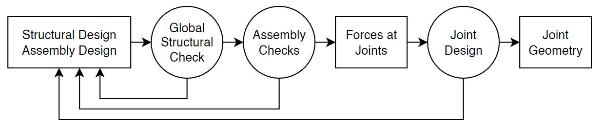
\includegraphics[width=15.92cm,height=14.36cm]{./images/image3.jpeg}
\end{figure}


This software arrangement with an overarching process execution controller is generic for any multi-controller scenarios. Level 1 or Level 2 controllers can be added if additional hardware is needed for the process. In this case, the Level 3 Process Execution Controller only needs to be revised to manage the new connection and to support the new commands \textit{(see \uline{6.3.8 Standalone Process Execution Controller})}. 

Experience has shown that the use of compas\_rrc \href{https://www.zotero.org/google-docs/?svtqbp}{(Fleischmann et al., 2020)} to send commands between Levels 2 and 3 is extremely flexible. Specifically, the `Instructions` class can be used to encapsulate newly developed instruction sets, such as requesting a status report, setting states, or starting an action. It also supports synchronous and asynchronous command modes, which is essential for managing long-running motion tasks. In addition, the use of ROS messaging system by compas\_fab allows easy addition of Level 2 controllers, even if they are running on a different computer. 

\section{Conclusion of Discussion}

In conclusion, this chapter has offered new insights into the automatic timber frame assembly problem and highlighted the discoveries that are relevant beyond the initial scope. Throughout the chapter, several areas have been identified where the DiRT timber assembly system could be improved to increase reliability, flexibility and efficiency. The discussion also covered how the DiRT concept could be implemented on future construction sites and generalised for other construction systems. 

In some parts, the research has reached limits of what can be done within the scope of the assembly process and further progress has to be made together with upstream and downstream construction partners. This chapter has also raised many new challenges, questions and unexplored knowledge gaps that require the involvement of various domain experts. Future research should concentrate on fostering interdisciplinary collaborations to develop innovative solutions for these challenges.
